\documentclass[tikz,border=6pt]{standalone}
\usepackage[T1]{fontenc}
\usepackage[utf8]{inputenc}
\usepackage{pgfplots}
\usepgfplotslibrary{groupplots}
\usetikzlibrary{calc}
\pgfplotsset{compat=1.18}
\begin{document}
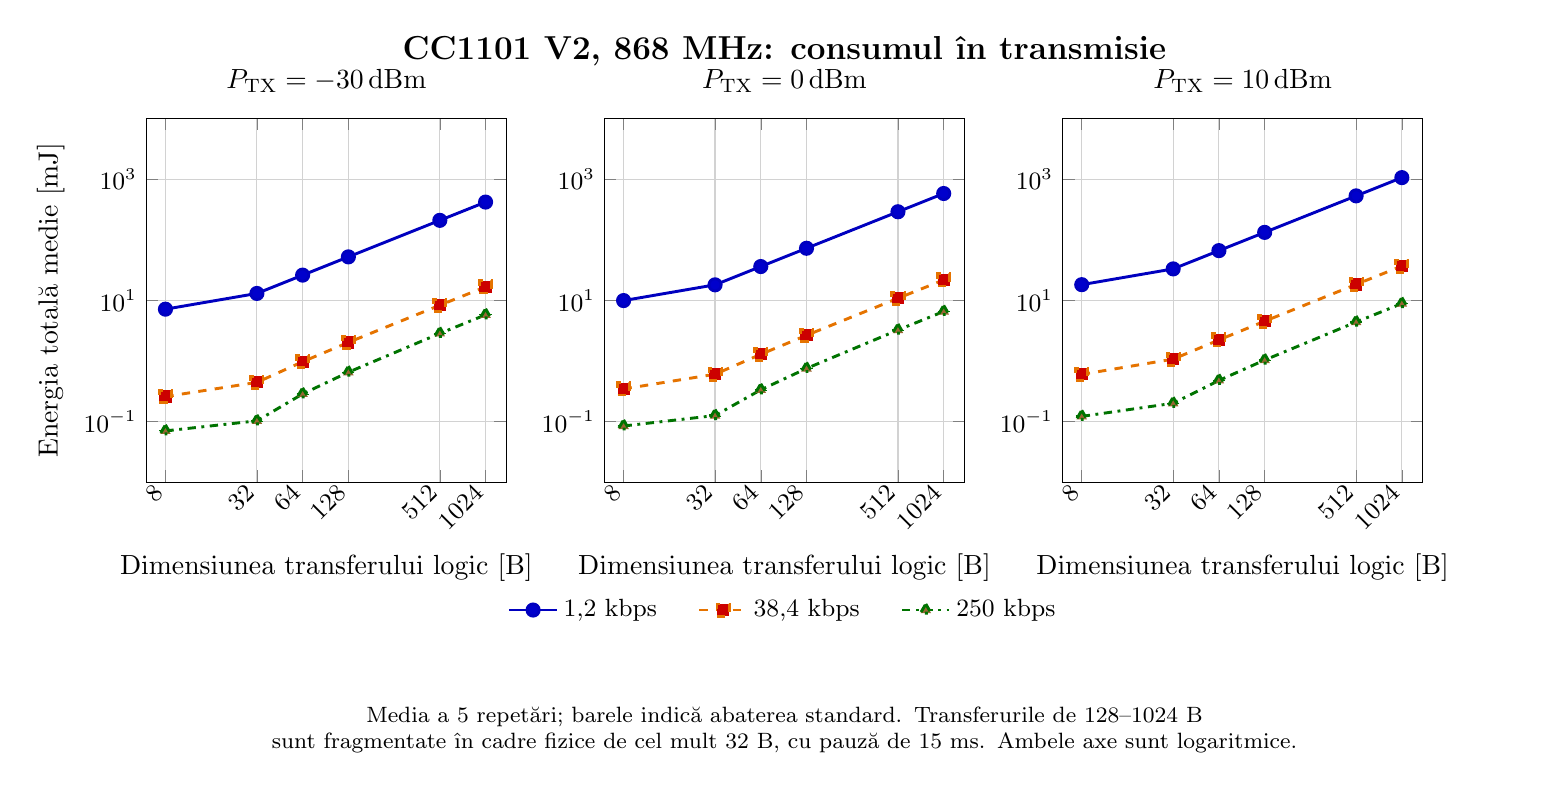
\begin{tikzpicture}
\begin{groupplot}[/pgf/number format/use comma,
  group style={group size=3 by 1, horizontal sep=1.25cm},
  width=6.15cm, height=6.2cm,
  xmode=log, log basis x={2},
  ymode=log, log basis y={10},
  ymin=0.01, ymax=10000,
  xmin=6, xmax=1400,
  xtick={8,32,64,128,512,1024},
  xticklabels={8,32,64,128,512,1024},
  x tick label style={rotate=45, anchor=east, font=\small},
  y tick label style={font=\small},
  grid=both, minor grid style={gray!15}, major grid style={gray!35},
  xlabel={Dimensiunea transferului logic [B]},
  every axis plot/.append style={line width=1.05pt},
  error bars/error bar style={line width=0.35pt},
  legend style={font=\small, draw=none, fill=none,
    at={(0.5,-0.29)}, anchor=north, legend columns=3,
    /tikz/every even column/.append style={column sep=0.45cm}},
]
\nextgroupplot[title={\(P_{\mathrm{TX}}=-30\,\mathrm{dBm}\)}, ylabel={Energia totală medie [mJ]}]
\addplot+[
  color=blue!75!black, solid, mark=*, mark size=2.2pt,
  error bars/.cd, y dir=both, y explicit,
] coordinates {
  (8,7.16890594) +- (0,0.0221462215)
  (32,13.0289909) +- (0,0.00495337561)
  (64,26.1289482) +- (0,0.0133697467)
  (128,52.3068621) +- (0,0.0262266361)
  (512,209.409263) +- (0,0.107627036)
  (1024,419.13487) +- (0,0.289155713)
};
\addplot+[
  color=orange!90!black, dashed, mark=square*, mark size=2.2pt,
  error bars/.cd, y dir=both, y explicit,
] coordinates {
  (8,0.259029957) +- (0,0.00254559931)
  (32,0.444195379) +- (0,0.00227012182)
  (64,0.973834894) +- (0,0.00442414915)
  (128,2.02742953) +- (0,0.00539681781)
  (512,8.32493111) +- (0,0.00795038518)
  (1024,16.7219755) +- (0,0.0206500783)
};
\addplot+[
  color=green!45!black, dashdotted, mark=triangle*, mark size=2.2pt,
  error bars/.cd, y dir=both, y explicit,
] coordinates {
  (8,0.0703318298) +- (0,0.00214527495)
  (32,0.103036729) +- (0,0.00195118942)
  (64,0.286387314) +- (0,0.00248888883)
  (128,0.653405084) +- (0,0.00396453434)
  (512,2.85133696) +- (0,0.00573648512)
  (1024,5.78560861) +- (0,0.00397146402)
};
\nextgroupplot[title={\(P_{\mathrm{TX}}=0\,\mathrm{dBm}\)}]
\addplot+[
  color=blue!75!black, solid, mark=*, mark size=2.2pt,
  error bars/.cd, y dir=both, y explicit,
] coordinates {
  (8,9.93845849) +- (0,0.00432399201)
  (32,18.0794873) +- (0,0.0222865273)
  (64,36.2130194) +- (0,0.0176486352)
  (128,72.5234932) +- (0,0.0265486404)
  (512,290.155191) +- (0,0.113563972)
  (1024,580.514158) +- (0,0.189795513)
};
\addlegendentry{1{,}2 kbps}
\addplot+[
  color=orange!90!black, dashed, mark=square*, mark size=2.2pt,
  error bars/.cd, y dir=both, y explicit,
] coordinates {
  (8,0.346322321) +- (0,0.00383679244)
  (32,0.60510309) +- (0,0.00175838749)
  (64,1.29083371) +- (0,0.00377714874)
  (128,2.65449617) +- (0,0.00395274518)
  (512,10.8465079) +- (0,0.00306916221)
  (1024,21.7636249) +- (0,0.0201489929)
};
\addlegendentry{38{,}4 kbps}
\addplot+[
  color=green!45!black, dashdotted, mark=triangle*, mark size=2.2pt,
  error bars/.cd, y dir=both, y explicit,
] coordinates {
  (8,0.0847533272) +- (0,0.00228107481)
  (32,0.12603198) +- (0,0.00285615413)
  (64,0.334783213) +- (0,0.00443801273)
  (128,0.753868789) +- (0,0.00347418685)
  (512,3.24698553) +- (0,0.00495807092)
  (1024,6.57189507) +- (0,0.0039360263)
};
\addlegendentry{250 kbps}
\nextgroupplot[title={\(P_{\mathrm{TX}}=10\,\mathrm{dBm}\)}]
\addplot+[
  color=blue!75!black, solid, mark=*, mark size=2.2pt,
  error bars/.cd, y dir=both, y explicit,
] coordinates {
  (8,18.1883048) +- (0,0.0177717961)
  (32,33.1117291) +- (0,0.0183400067)
  (64,66.2888726) +- (0,0.0194064677)
  (128,132.58372) +- (0,0.0251988428)
  (512,530.491757) +- (0,0.151785874)
  (1024,1061.48675) +- (0,0.313866891)
};
\addplot+[
  color=orange!90!black, dashed, mark=square*, mark size=2.2pt,
  error bars/.cd, y dir=both, y explicit,
] coordinates {
  (8,0.602501373) +- (0,0.00267156186)
  (32,1.07354411) +- (0,0.00317321951)
  (64,2.2285692) +- (0,0.006435654)
  (128,4.53645395) +- (0,0.00376653717)
  (512,18.3660392) +- (0,0.010287699)
  (1024,36.7936547) +- (0,0.00554884912)
};
\addplot+[
  color=green!45!black, dashdotted, mark=triangle*, mark size=2.2pt,
  error bars/.cd, y dir=both, y explicit,
] coordinates {
  (8,0.122087858) +- (0,0.0020178284)
  (32,0.2008944) +- (0,0.000923412057)
  (64,0.478253901) +- (0,0.0032034274)
  (128,1.03680708) +- (0,0.00397707218)
  (512,4.39720427) +- (0,0.00166498845)
  (1024,8.87376302) +- (0,0.00901416598)
};
\end{groupplot}
\node[font=\bfseries\large] at ($(group c2r1.north)+(0,0.85cm)$)
  {CC1101 V2, 868 MHz: consumul în transmisie};
\node[font=\footnotesize, align=center, text width=18.5cm]
  at ($(group c2r1.south)+(0,-3.15cm)$)
  {Media a 5 repetări; barele indică abaterea standard. Transferurile de 128--1024 B\\
   sunt fragmentate în cadre fizice de cel mult 32 B, cu pauză de 15 ms. Ambele axe sunt logaritmice.};
\end{tikzpicture}
\end{document}
